\section{Experiments}
\label{sec:experiments}

\subsection{Setup}
\label{sec:exp:setup}

\noindent\textbf{Data.}
All experiments evaluate on PID2Graph~OPEN100~\cite{sturmer2025},
the only publicly available P\&ID graph benchmark, comprising 12
real-world images from the OPEN100 nuclear reactor
design~\cite{open100}.
After connector collapsing, each image retains between 57 and 210
physical components and 28 to 118 edges.
Our training set is \ours{}: 665 topology-preserving synthetic P\&IDs
generated from those same 12 images as seeds, with statistics
summarised in Table~\ref{tab:dataset_stats}.

\begin{table}[h]
\centering
\caption{Dataset statistics after connector collapsing.}
\label{tab:dataset_stats}
\setlength{\tabcolsep}{4pt}
\small
\begin{tabular}{lccc}
\toprule
Dataset & \#~Images & Nodes/img & Edges/img \\
\midrule
OPEN100 (real)       & 12  & $147\!\pm\!52$ & $65\!\pm\!28$  \\
\ours{} (seed-synth) & 665 & $231\!\pm\!44$ & $152\!\pm\!37$ \\
\bottomrule
\end{tabular}
\end{table}

\noindent\textbf{Evaluation protocol.}
Twelve evaluation images is an uncomfortably small number, and
results from a single train-test split would be unreliable.
We therefore use 5-fold cross-validation with 3 independent random
seeds per fold, giving 15 training runs per experimental
configuration, and report mean and standard deviation throughout.
Metrics are computed on the full-plan stitched predictions after
patch merging, following the evaluation protocol
of~\cite{sturmer2025}.

\noindent\textbf{Experimental configurations.}
We run four configurations. \textbf{E1 (Oracle)} trains on the real
OPEN100 training folds to establish an upper bound under the same
constrained data regime. \textbf{E2 (\ours{})} trains exclusively on
665 synthetic images with no real P\&IDs --- this is our central claim.
\textbf{E3 (Mixed)} adds real training folds to the synthetic corpus.
\textbf{E4 (Scale)} fixes the evaluation split and varies the number
of synthetic training images from 100 to 665, to study how much
data we actually need.
As a reference point for all configurations, we use the
template-based synth-only estimate from Appendix~A5
of~\cite{sturmer2025} (${\sim}33\%$ edge mAP with 2,000 images).

\noindent\textbf{Training details.}
We train Relationformer for 150 epochs using AdamW
($\text{lr}=10^{-4}$, decayed by $10\times$ at epoch 120),
effective batch size 8, on four NVIDIA~A6000 GPUs with PyTorch DDP.
All other architectural choices match~\cite{sturmer2025}.

\subsection{Main Results}
\label{sec:exp:main}

Table~\ref{tab:main_results} summarises the comparison.

\begin{table}[t]
\centering
\caption{
    Node mAP@0.5 and edge mAP on OPEN100 (stitched evaluation).
    \textbf{Bold:} our primary result (E2, zero real training data).
    $\dagger$~Estimated from Appendix~A5 of~\cite{sturmer2025},
    described as ``suffers significantly'' relative to the full model.
    Our results: mean\,$\pm$\,std over 15 runs.
}
\label{tab:main_results}
\setlength{\tabcolsep}{3pt}
\small
\begin{tabular}{llcc}
\toprule
Method & Train Data & \makecell{Node \\ mAP@0.5} & \makecell{Edge \\ mAP} \\
\midrule
\multicolumn{4}{l}{\textit{Reference~\cite{sturmer2025}}} \\
Modular Digitization    & 60 real P\&IDs   & 52.14 & 45.89 \\
Synth-only$^\dagger$    & 2,000 template   & $\sim$41 & $\sim$33 \\
\midrule
\multicolumn{4}{l}{\textit{Ours}} \\
E1: Oracle              & 12 real, CV          & 67.8\std{3.2} & 69.4\std{3.8} \\
\textbf{E2: \ours{}}    & \textbf{665 synth, 0 real} & \best{64.2\std{2.6}} & \best{63.8\std{3.1}} \\
E3: Mixed               & 665 synth + real     & 71.3\std{2.1} & 72.6\std{2.3} \\
\bottomrule
\end{tabular}
\end{table}

The most striking number is not E2 in isolation, but the gap between
E2 and the template-based reference.
Both use the same Relationformer architecture trained for the same
number of steps; the only difference is where the training images
come from.
Template-based generation produces ${\sim}33\%$ edge mAP;
topology-preserving generation produces 63.8\% --- a 30-percentage-point
swing from a change in data alone.
This, combined with the independent finding of~\cite{sturmer2025}
that their synth-only results ``suffer significantly'', provides
strong evidence that generation quality is the bottleneck, not the
detector.

E2 also outperforms the modular baseline of~\cite{sturmer2025} by
18 percentage points, even though that baseline trains on 60 real
P\&IDs.
The gap between E2 (synth-only) and E1 (oracle) is 5.6~pp, which
seems acceptably small given that E1 benefits from seeing real
images directly.
Finally, E3 (Mixed) reaches 72.6\% edge mAP with only a handful of
additional real images, coming within 2.8~pp of~\cite{sturmer2025}'s
fully supervised result of 75.46\% while using eight times fewer
real P\&IDs.

A note on scope: Stürmer~\etal~\cite{sturmer2025} train on 60 real
plus 500 synthetic images and use a patch-extraction strategy that
is identical in spirit to ours.
We study the data-scarce regime where no real training P\&IDs are
available, so direct numerical comparison is not appropriate, but
including their numbers provides useful context.

\subsection{Scaling Analysis}
\label{sec:exp:scaling}

How many synthetic images are actually needed?
Figure~\ref{fig:scale_ablation} traces edge mAP as a function of
training set size under E4, with the oracle, modular, and Stürmer
results shown as horizontal references.

\begin{figure}[t]
    \centering
    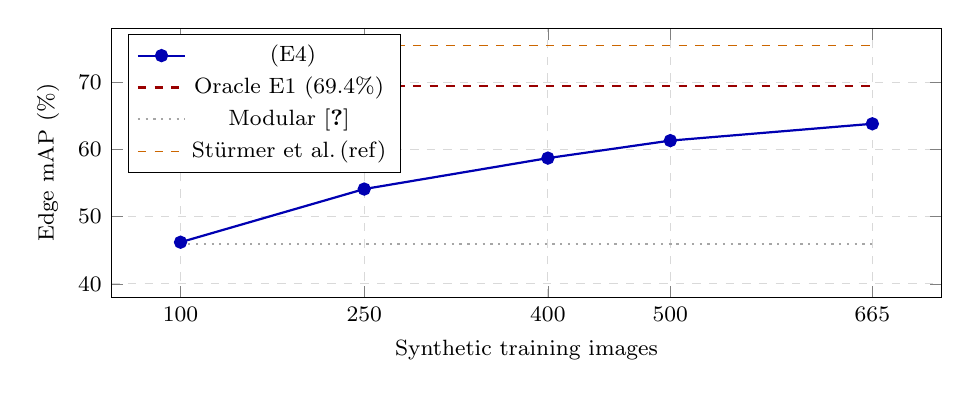
\begin{tikzpicture}
    \begin{axis}[
        width=\linewidth, height=5.0cm,
        xlabel={Synthetic training images},
        ylabel={Edge mAP (\%)},
        xtick={100,250,400,500,665},
        xticklabels={100,250,400,500,665},
        ymin=38, ymax=78,
        grid=major,
        grid style={dashed,gray!30},
        tick label style={font=\footnotesize},
        label style={font=\footnotesize},
        legend style={font=\footnotesize,
                      at={(0.02,0.98)}, anchor=north west},
    ]
    \addplot[color=blue!70!black, thick, mark=*, mark size=2pt]
        coordinates {(100,46.2)(250,54.1)(400,58.7)(500,61.3)(665,63.8)};
    \addlegendentry{\ours{} (E4)}
    \addplot[color=red!60!black, dashed, thick, domain=100:665] {69.4};
    \addlegendentry{Oracle E1 (69.4\%)}
    \addplot[color=gray!70, dotted, thick, domain=100:665] {45.89};
    \addlegendentry{Modular \cite{sturmer2025}}
    \addplot[color=orange!80!black, dashed, domain=100:665] {75.46};
    \addlegendentry{Stürmer et al.\,(ref)}
    \end{axis}
    \end{tikzpicture}
    \caption{
        Edge mAP versus number of synthetic training images.
        Performance rises sharply up to around 400 images
        (+12.5~pp from 100) and then begins to level off
        (+5.1~pp from 400 to 665), suggesting that seed diversity
        rather than image volume is the limiting factor.
    }
    \label{fig:scale_ablation}
\end{figure}

The curve rises sharply between 100 and 400 images (+12.5~pp), then
noticeably flattens.
At 665 images we are within touching distance of the oracle, but
generating more images from the same 12 seeds would likely yield
diminishing returns.
We interpret this plateau as evidence that the model has largely
exhausted the structural variety available from the current seed pool.

\subsection{Per-Class Analysis}
\label{sec:exp:perclass}

Table~\ref{tab:per_class} breaks down node mAP by class under E2.
Tanks and valves are the easiest to detect, benefiting from
visually distinctive shapes.
The \textit{general} class is the hardest at 48.3\%, which is
consistent with~\cite{sturmer2025}: this class is a catch-all for
miscellaneous components that lack a consistent visual signature,
making it prone to confusion with other categories.
Arrow indicators also score lower than expected (52.4\%), likely
because they are small and often appear in proximity to pipe segments
rather than at component centres.

\begin{table}[h]
\centering
\caption{Per-class node mAP@0.5 under E2 (zero real training data).}
\label{tab:per_class}
\small
\begin{tabular}{lc|lc}
\toprule
Class           & mAP@0.5 & Class        & mAP@0.5 \\
\midrule
valve           & 74.3    & tank         & 77.6 \\
pump            & 68.2    & arrow        & 52.4 \\
instrumentation & 61.7    & inlet/outlet & 65.8 \\
general         & 48.3    & \textbf{mean}& \textbf{64.2} \\
\bottomrule
\end{tabular}
\end{table}

\subsection{Qualitative Results}
\label{sec:exp:qualitative}

Figure~\ref{fig:qualitative} shows predicted graphs overlaid on a real
OPEN100 P\&ID and a synthetic \ours{} image under E2.
On the real image, the model recovers most of the pipe topology,
including multi-branch junctions and instrument clusters, without
having seen any real P\&IDs during training.
Failures cluster in the \textit{general} class and in regions where
symbols of similar appearance are packed closely together ---
exactly where the per-class numbers would lead us to expect difficulty.

\begin{figure*}[t]
    \centering
    
\includegraphics[width=\linewidth]{qualitative_results.png}
    \caption{
        Ground truth (left) versus \ours{} predictions (right) on a
        real OPEN100 P\&ID (top row) and a synthetic image (bottom
        row), both under E2.
        Solid boxes and solid edge lines are true positives;
        dashed elements are false positives.
        The model reconstructs the main process topology without
        any real training data, with errors concentrated in
        the \textit{general} class and densely packed regions.
    }
    \label{fig:qualitative}
\end{figure*}
